%!/usr/bin/env pdflatex
%-*- coding: utf-8 -*-
%@author : Romain Graux
%@date : 2022 Mar 08, 16:20:03
%@last modified : 2022 Mar 15, 19:43:16


% [ PLAN ] 
% - Motivation
%   - Classical compressors (JPEG, ...)
%   - What we need (tasks)
%   - What they built
% - Intuition
%   - Example on MNIST

\documentclass[10pt,t]{beamer}


% Import all packages
\usepackage{graphicx,xcolor,caption}

% Color declarations
\definecolor{greyBackgroundColor}{rgb}{0.8,0.8,0.8}
\definecolor{primaryColor}{rgb}{0.5,0,0.5}
\definecolor{secondaryColor}{rgb}{0,0,0}

% Theme definition and progessbar settings
\usetheme[progressbar=frametitle]{metropolis}
\setbeamertemplate{frame numbering}[fraction]

% Settings of all colors
\setbeamercolor{background canvas}{bg=white}
\setbeamercolor{title}{fg=primaryColor}
\setbeamercolor{frametitle}{bg=greyBackgroundColor, fg=primaryColor}
\setbeamercolor{structure}{fg=primaryColor}
\setbeamercolor{subsection in head/foot}{fg=secondaryColor}
\setbeamercolor{progress bar}{fg=secondaryColor}

% Personal commands declaration
% all path commands
\newcommand{\docsPath}[1]{./docs/#1}
\newcommand{\imgsPath}[1]{\docsPath{imgs/#1}}
\newcommand{\mnistPath}[1]{\imgsPath{mnist/#1}}
% visualization commands
\newcommand{\question}[1]{\colorbox{primaryColor!15}{\large{\color{secondaryColor}#1}}}

% Meta information declaration
\title{Lossy compression for lossless prediction}
\subtitle{EECS Seminar: Advanced Topics in Machine Learning}
\author{Romain Graux}
\date{\today}

\begin{document}
\metroset{block=fill}

\begin{frame}
    \titlepage
\end{frame}

\begin{frame}{Motivation}
    $10^{21}$ - $10^{23}$ bytes data collected per year

    \only<2->{
        $\rightarrow$ But most data is processed by algorithms performing \textbf{downstream tasks}.
    \vspace{5pt}
    }

    \def \imgWidth {0.23\textwidth}
    

    \only<3>{
        \begin{figure}
            \centering
            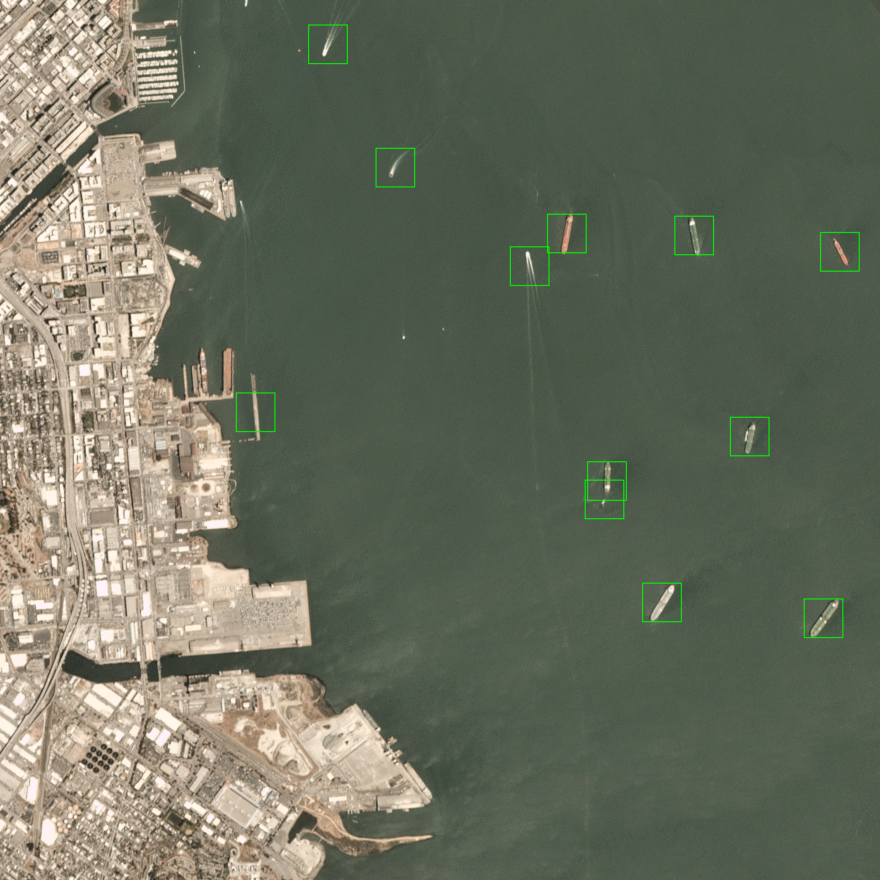
\includegraphics[width=\imgWidth]{\imgsPath{applications/satellite-detection.png}} \quad
            \includegraphics[width=\imgWidth]{\imgsPath{void.png}} \\
            \includegraphics[width=\imgWidth]{\imgsPath{void.png}} \quad
            \includegraphics[width=\imgWidth]{\imgsPath{void.png}} 
        \end{figure}
    }

    \only<4>{
        \begin{figure}
            \centering
            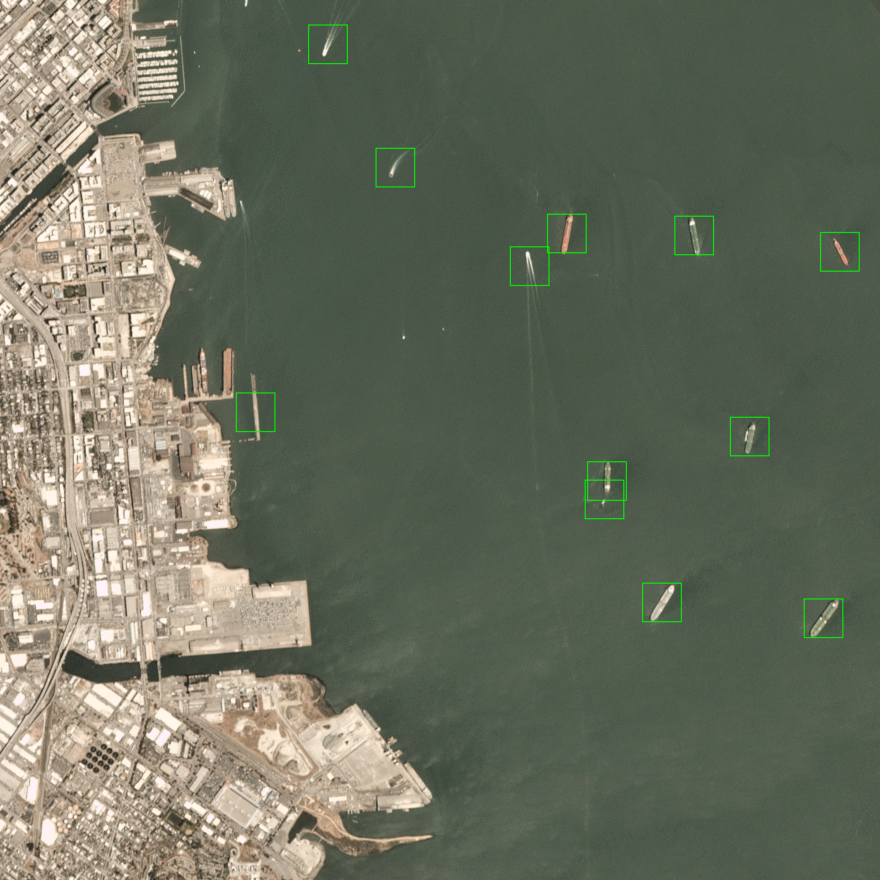
\includegraphics[width=\imgWidth]{\imgsPath{applications/satellite-detection.png}} \quad
            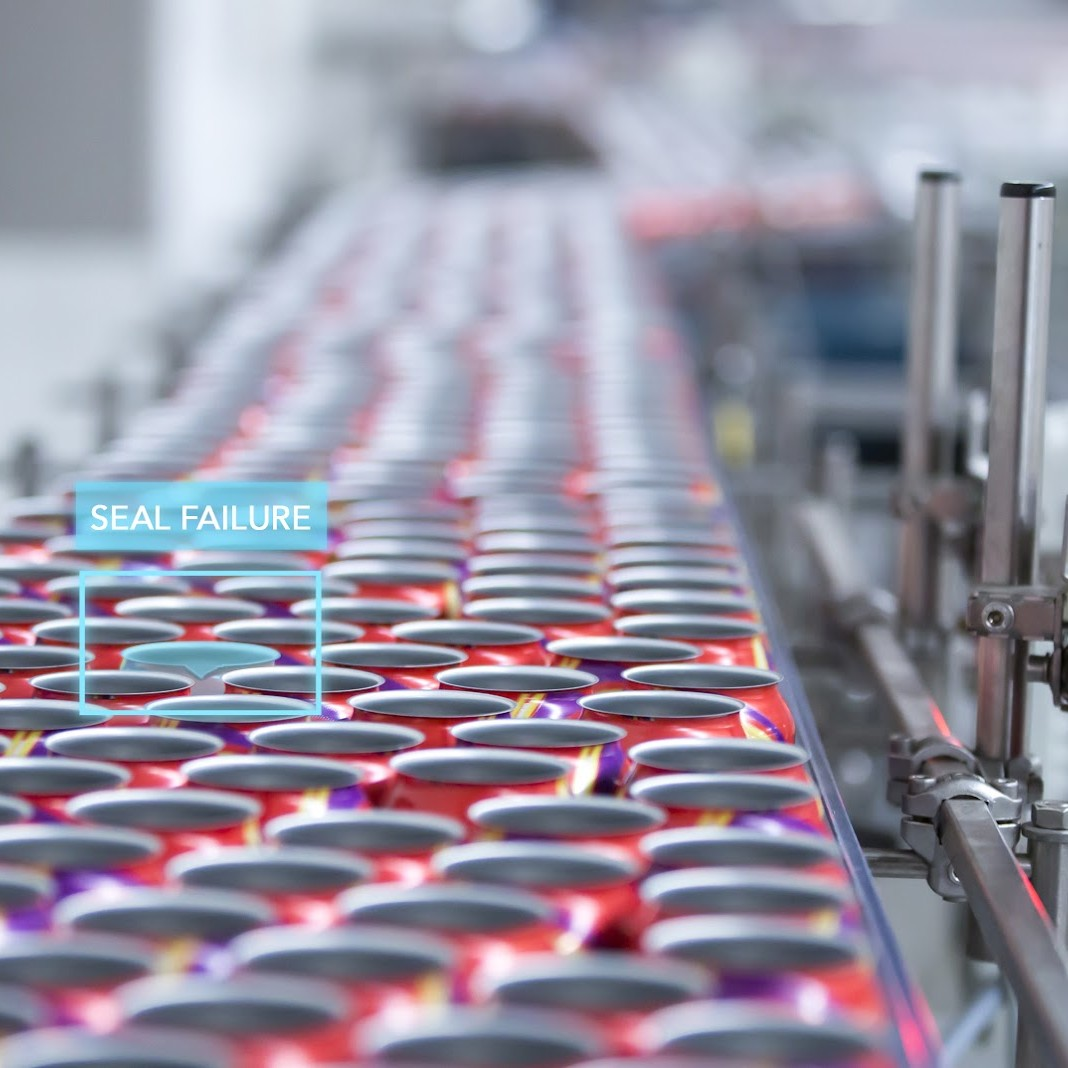
\includegraphics[width=\imgWidth]{\imgsPath{applications/quality_control.jpg}} \\
            \includegraphics[width=\imgWidth]{\imgsPath{void.png}} \quad
            \includegraphics[width=\imgWidth]{\imgsPath{void.png}} 
        \end{figure}
    }

    \only<5>{
        \begin{figure}
            \centering
            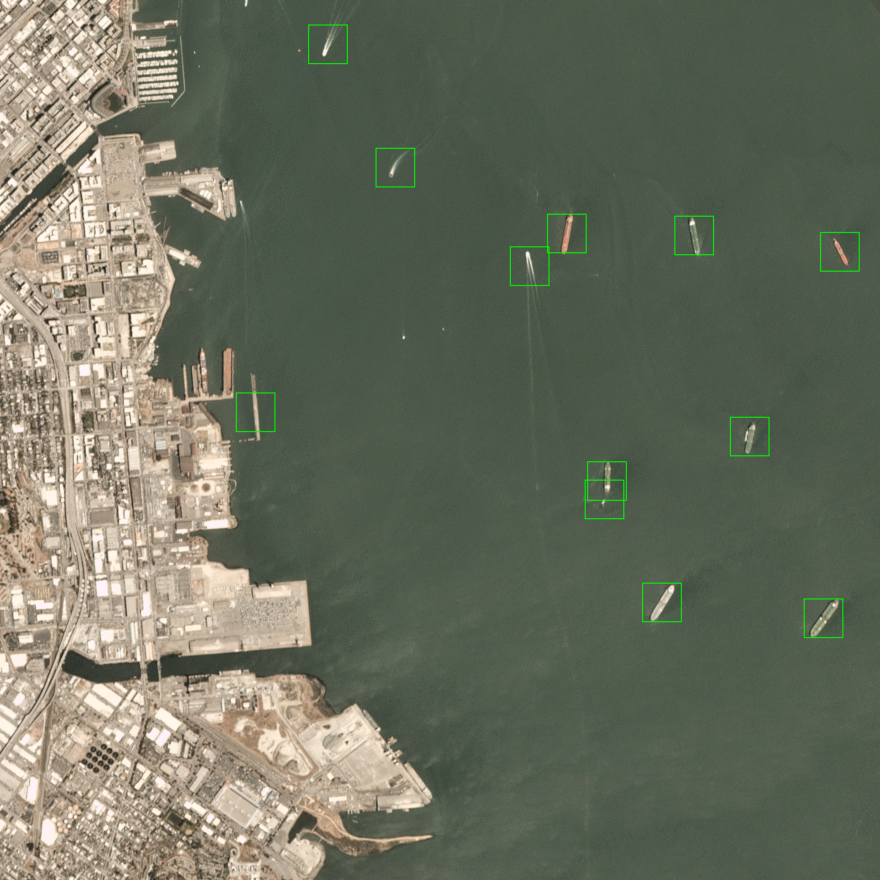
\includegraphics[width=\imgWidth]{\imgsPath{applications/satellite-detection.png}} \quad
            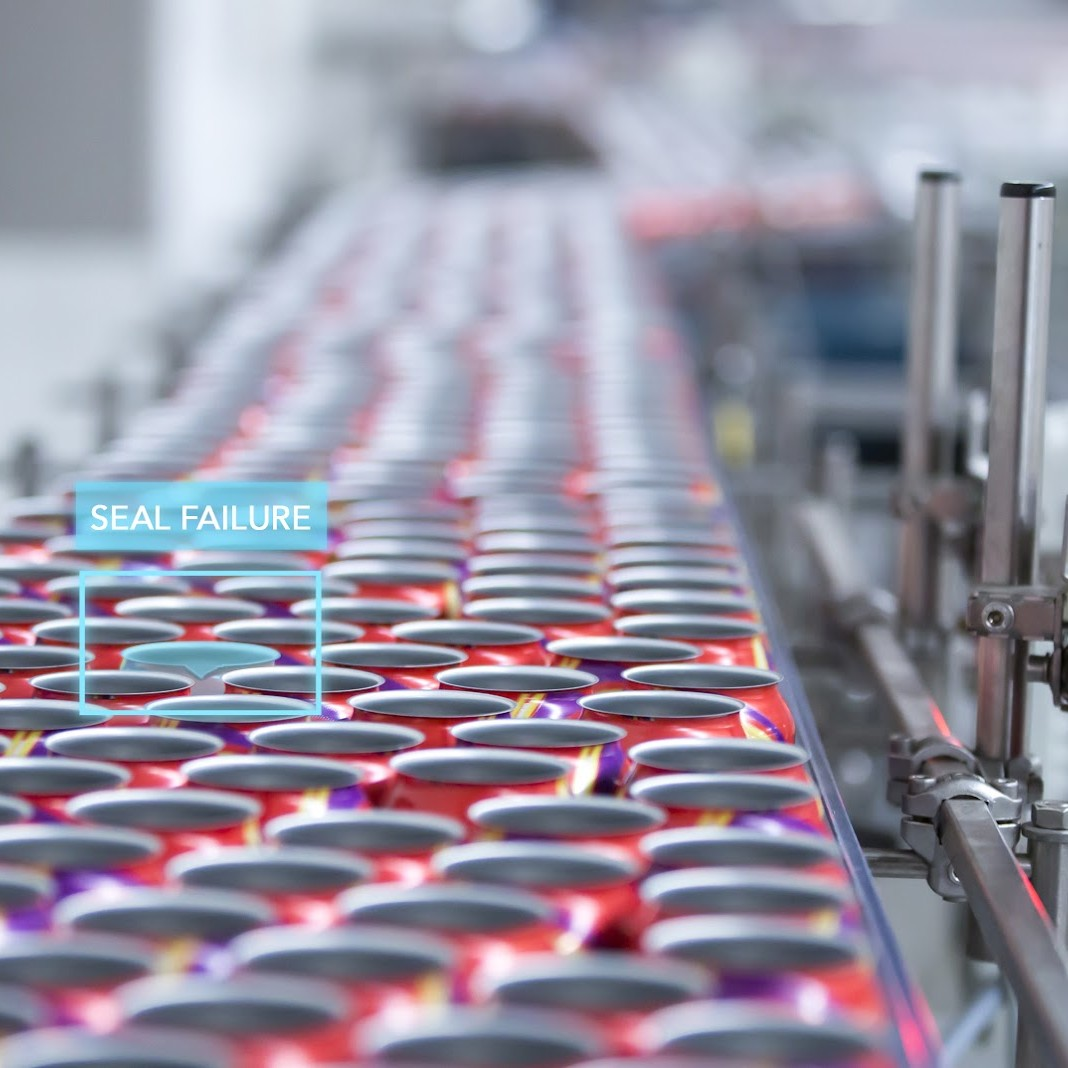
\includegraphics[width=\imgWidth]{\imgsPath{applications/quality_control.jpg}} \\[12pt]
            \includegraphics[width=\imgWidth]{\imgsPath{void.png}} \quad
            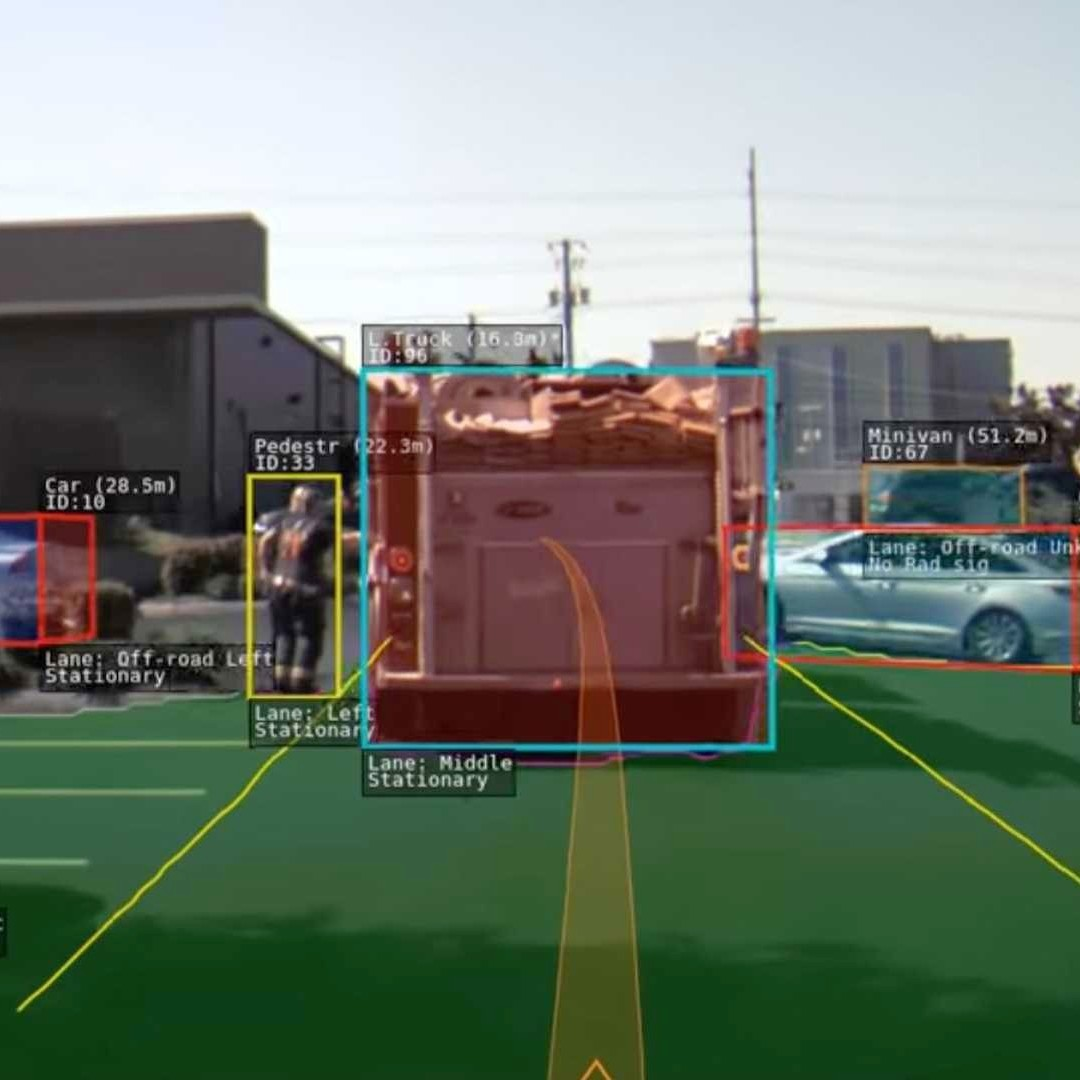
\includegraphics[width=\imgWidth]{\imgsPath{applications/selfdriving-cars.jpeg}} 
        \end{figure}
    }

    \only<6>{
        \begin{figure}
            \centering
            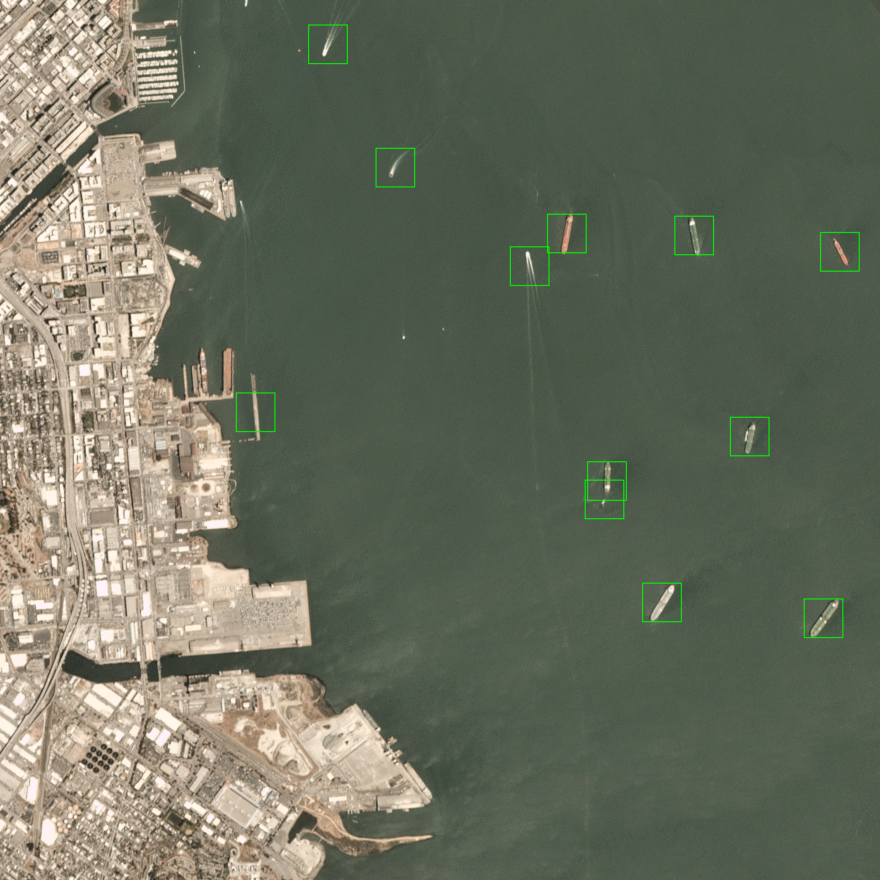
\includegraphics[width=\imgWidth]{\imgsPath{applications/satellite-detection.png}} \quad
            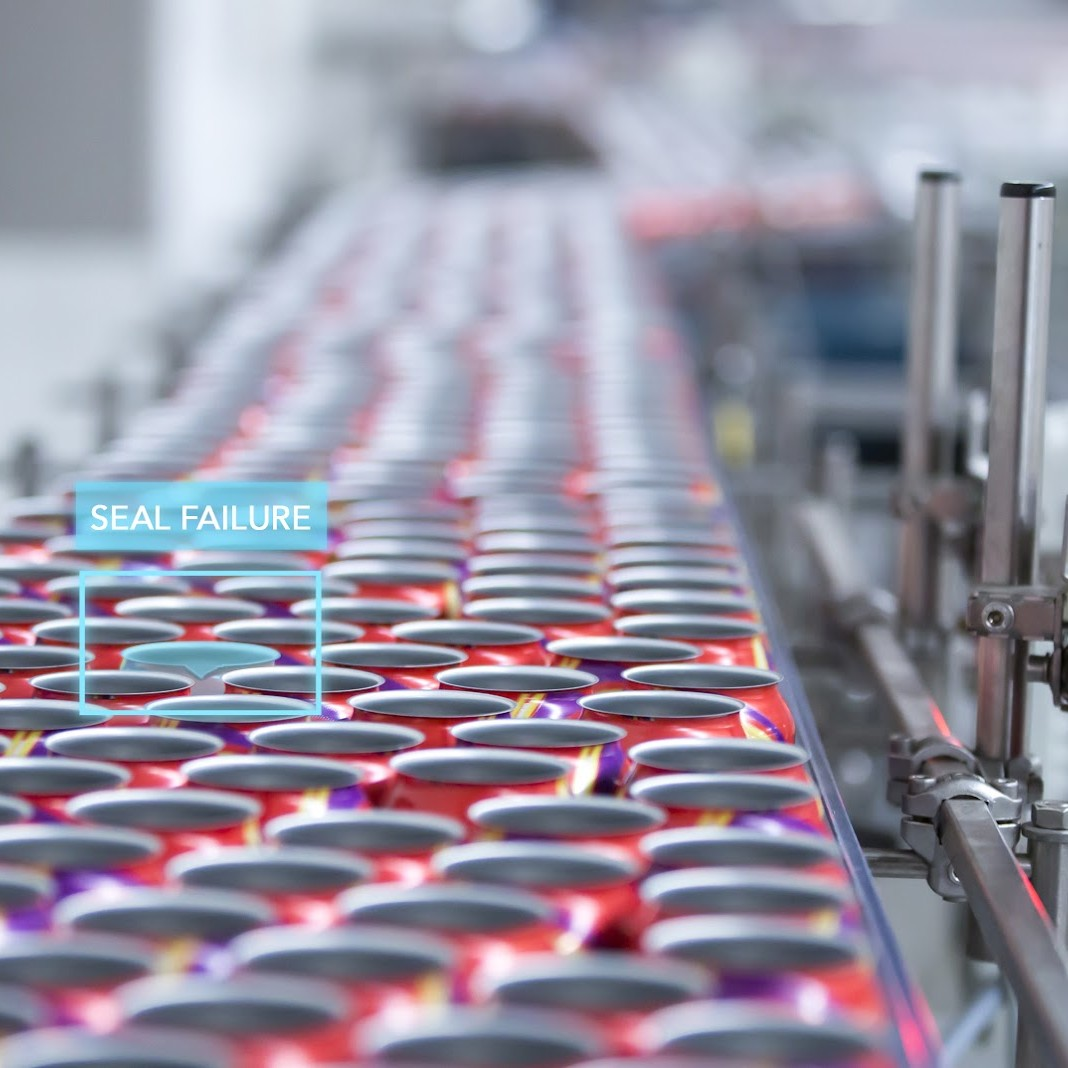
\includegraphics[width=\imgWidth]{\imgsPath{applications/quality_control.jpg}} \\[12pt]
            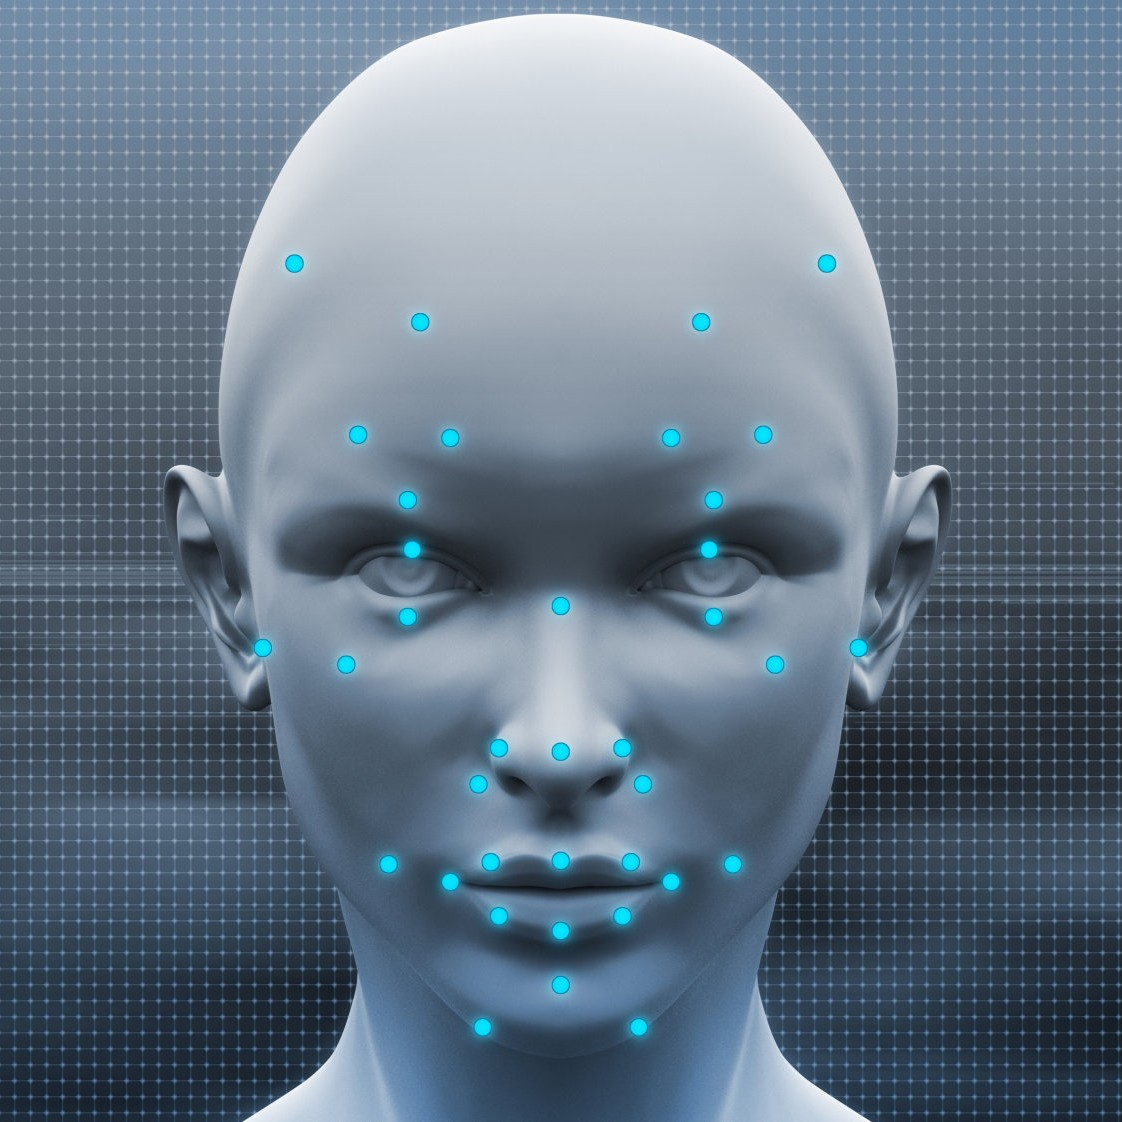
\includegraphics[width=\imgWidth]{\imgsPath{applications/face-recognition.jpeg}} \quad
            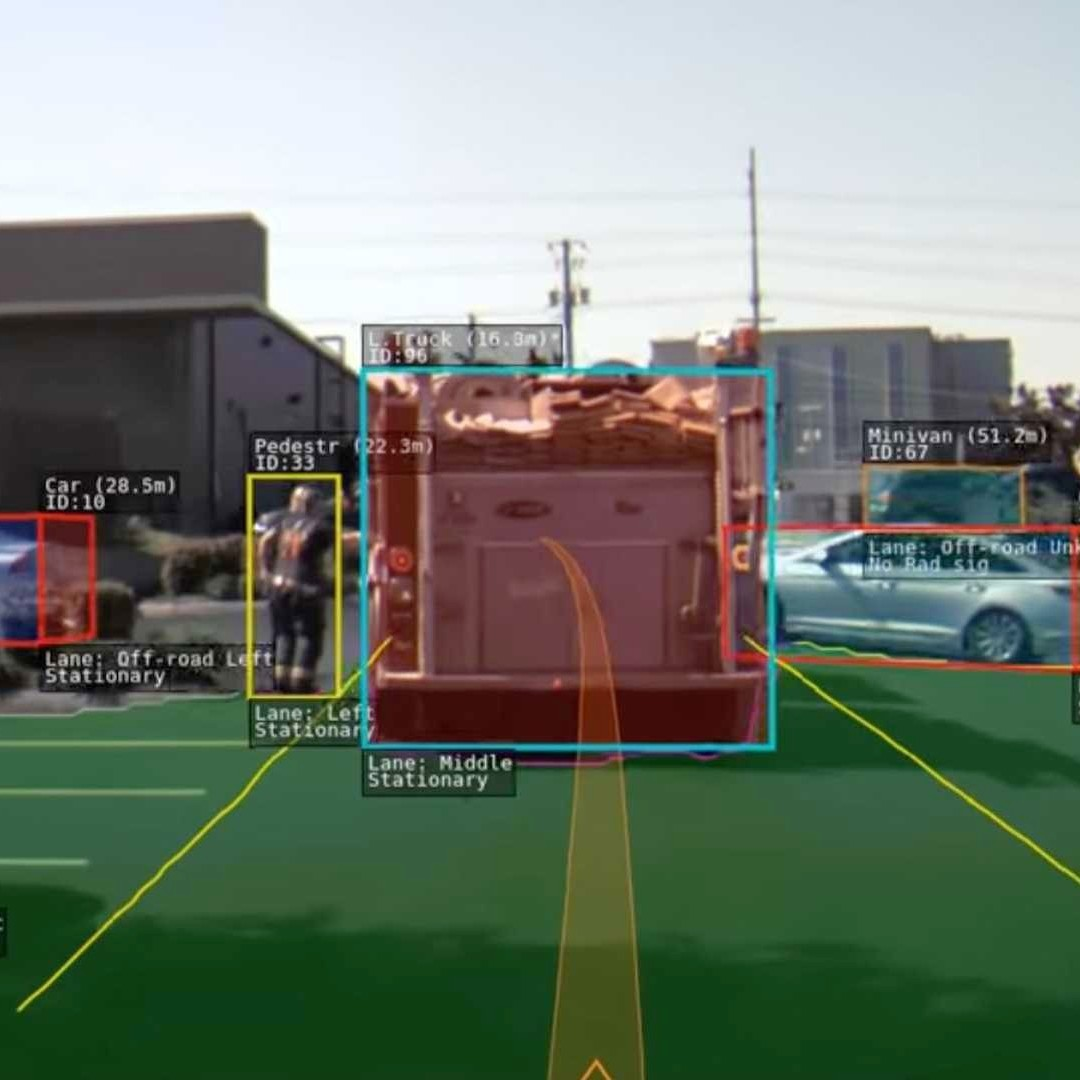
\includegraphics[width=\imgWidth]{\imgsPath{applications/selfdriving-cars.jpeg}} 
        \end{figure}
    }

    \only<7->{
        Yet current compressors optimize high \textbf{perceptual} fidelity
    }

    \only<8->{
        \begin{itemize}
            \item Stores too much not needed information
            \item Does not ensure good task performance
        \end{itemize}
    }


    \vfill
    \begin{columns}
    \column{0.2\textwidth}
    \only<9->{
            \begin{figure}
                \centering
                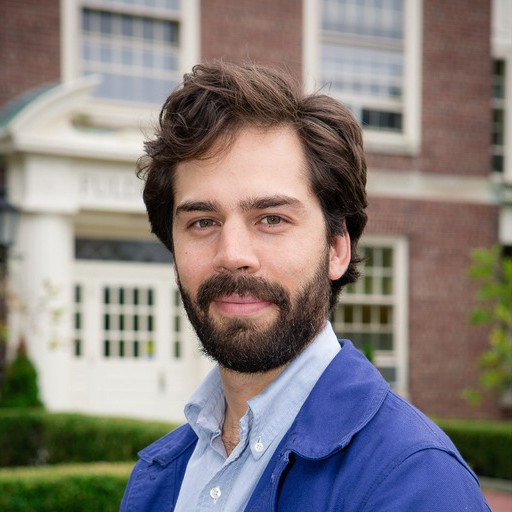
\includegraphics[width=\textwidth]{\imgsPath{chris/source.jpeg}}
                \caption*{Source}
                \label{fig:chris-source}
            \end{figure}
    }

    \column{0.2\textwidth}
    \only<10->{
            \begin{figure}
                \centering
                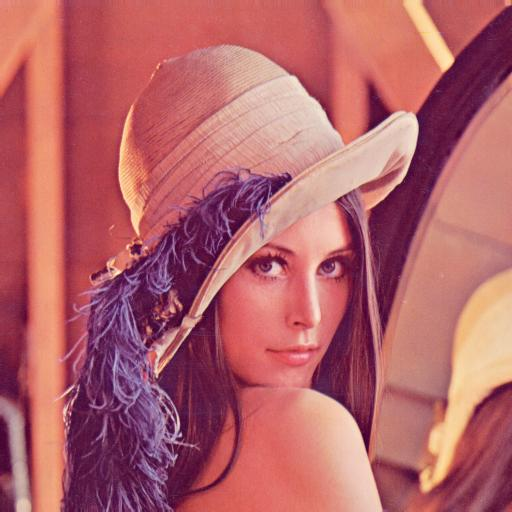
\includegraphics[width=\textwidth]{\imgsPath{chris/high.jpeg}}
                \caption*{High bitrate}
                \label{fig:chris-high}
            \end{figure}
    }

    \column{0.2\textwidth}
    \only<11->{
            \begin{figure}
                \centering
                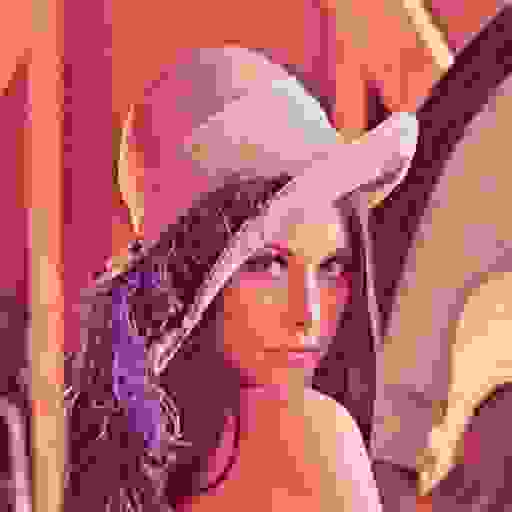
\includegraphics[width=\textwidth]{\imgsPath{chris/low.jpeg}}
                \caption*{Low bitrate}
                \label{fig:chris-low}
            \end{figure}
    }

    \column{0.2\textwidth}
    \only<12->{
            \begin{figure}
                \centering
                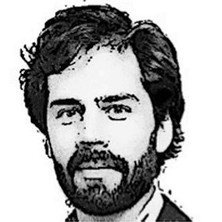
\includegraphics[width=\textwidth]{\imgsPath{chris/desired.jpeg}}
                \caption*{Desired}
                \label{fig:chris-desired}
            \end{figure}
    }
    \end{columns}
\end{frame}

\begin{frame}{What they designed}
    \begin{center}
        \large{They designed a \textbf{task-centric} distortion that ensures good downstream performance}
    \end{center}
    \pause
    \vfill
    \begin{itemize}[<+->]
        \item Characterize minimum bit-rate to ensure high performance on desired tasks;
        \item Derive unsupervised objectives for training \textbf{task-centric} compressors;
        \item $> 1000x$ compression gains on Imagenet compared to JPEG (see Slide \ref{slide:performance}).
    \end{itemize}
\end{frame}

\begin{frame}{Intuition: Augmented MNIST}
    \foreach \dir\cap\lab in {
        \mnistPath{source/}/Source: Augmented MNIST/mnist-source,
        \mnistPath{standard/}/Standard neural compressor: 130 bit-rate/mnist-standard,
        \mnistPath{prototypicals/}/Their neural compressor: 48 bit-rate/mnist-our
    }{
        \only<1>{
            \begin{figure}
                \centering
                \includegraphics[width=0.15\textwidth]{\dir0.png}
                \includegraphics[width=0.15\textwidth]{\dir1.png}
                \includegraphics[width=0.15\textwidth]{\dir2.png}
                \includegraphics[width=0.15\textwidth]{\dir3.png}
                \includegraphics[width=0.15\textwidth]{\dir4.png}
                \caption*{\cap}
                \label{fig:\lab-big}
            \end{figure}

            \vspace{-15pt}
        }

        \only<2->{
            \begin{figure}
                \centering
                \includegraphics[width=0.05\textwidth]{\dir0.png}
                \includegraphics[width=0.05\textwidth]{\dir1.png}
                \includegraphics[width=0.05\textwidth]{\dir2.png}
                \includegraphics[width=0.05\textwidth]{\dir3.png}
                \includegraphics[width=0.05\textwidth]{\dir4.png}
                \label{fig:\lab-small}
            \end{figure}

            \vspace{-20pt}
        }
    }

    \only<2->{
        \vfill
        \textbf{Prototypical} digit ensures 
        \begin{math}
            \begin{array}{l}
                \rightarrow \text{high downstream performance}\\
                \rightarrow \text{good compression rate}
            \end{array}
        \end{math}
    }

    \only<3->{
        \vspace{5pt}
        \question{Why not sending directly the labels?}
    }

    \begin{itemize}
        \item<4-> Might be interested in multiple downstream tasks;
        \item<5-> Would require knowing tasks of interest at compression time.
    \end{itemize}

    \only<6->{
        $\rightarrow$ The objective is \textbf{unsupervised} 
    }

\end{frame}


\begin{frame}{Performance}
    \label{slide:performance}
\end{frame}

\end{document}

